% !Tex root = Vorlage.tex
Introduction text to our project.


\section{Minimum-Variance-Portfolio}
An investment strategy based on a Minimum Variance Portfolio seeks to minimize the risk of an investment. There is thus no desired target-return or stock-forecast to be considered. The portfolio optimization process can be described as pure risk-minimization, where the goal is a determination of the weight-distribution yielding the lowest possible risk at any time. Graphically, one can think of a Minimum Variance Portfolio as the most left point of the mean-variance-frontier.

\subsection{Theory}
As written in the paper by DeMiguel et al.\cite{DEM09}, the weights were chosen according to the portfolio that minimizes the variance of return, e.g. 

\begin{equation} \label{eq:1}
\min_{w_t} w_t^{\perp}\Sigma_{t}w_{t}
\end{equation}

under the restriction that 

\begin{equation} \label{eq:2}
1_{N}^{\perp}w_{t} \overset{!}{=} 1
\end{equation}

and

\begin{equation} \label{eq:3}
\Sigma_t w_t \overset{!}{=} 1,
\end{equation}

where $w_t \in \mathbb{R}^{N}$ is the weight-vector at time $t \in \lbrace 1, 2, \dots, T \rbrace$ with $T \in \mathbb{N}$ period under observation and $N \in \mathbb{N}$ number of assets considered. $\Sigma_t \in \mathbb{N \times N}$ names the covariance matrix of excess-returns $R_{\tau} \in \mathbb{R}^{N \times \tau}$ at time $t$ for a subset $\tau$ of the period of Observation $\tau \subseteq \lbrace 1, 2, \dots, T \rbrace$. In the equation above, 1 is thought of as the N-dimensional vector containing 1s. \\

We now want to investigate the restriction $\min_{w_t}$for one fixed time-period T, such that $\tau = T$. As a result, weights are not time-dependent anymore. Note that when constructing a Minimum Variance Portfolio, weights are in fact time-dependent. However, for the sake of legibility, we will for now treat the case where $w_t = w$.\\

Considering three risky assets and a weight vector $w \in \mathbb{R}^{3}$, such that 
\begin{equation}
  w = \begin{pmatrix}w_1\\w_2\\w_3\end{pmatrix},
\end{equation}
the minimal variance restraint can then be interpreted as follows\cite[p.~7]{ZIV13}:
\begin{equation} \label{eq:4}
  \begin{split}
    \min_{w_1, w_2, w_3} \sigma^2_{w_1, w_2, w_3} = & w^2_1 \sigma^2_1 + w^2_2 \sigma^2_2 + w^2_3 \sigma^2_3 + \\ & 2w_1w_2 \sigma_{12} + 2w_1w_3\sigma_{13} + 2w_2w_3\sigma_{23}
  \end{split}
\end{equation}
Here, the components' variance $\sigma^2_{i}$ and standard deviation $\sigma_{i,j}$ for $i,j \in \lbrace 1, 2, 3 \rbrace$ are used to describe the relationship. The Lagrange-function of this problem can be written as 
\begin{equation} \label{eq:5}
  \begin{split}
    L(w_1, w_2, w_3, \lambda) = & w^2_1 \sigma^2_1 + w^2_2 \sigma^2_2 + w^2_3 \sigma^2_3 + \\ & 2w_1w_2 \sigma_{12} + 2w_1w_3\sigma_{13} + 2w_2w_3\sigma_{23} \\
    + & \lambda(w_1 + w_2 + w_3 - 1)
  \end{split}
\end{equation}

Now, the component-wise deviates can be found and be set to equal zero, yielding the first order conditions.

\begin{equation} \label{eq:6}
  \begin{split}
    0 &= \frac{\partial L}{\partial w_1} = 2 w_1 \sigma^2_1 + 2 w_2 \sigma_{12} + 2 w_3 \sigma_{12} + \lambda \\
    0 &= \frac{\partial L}{\partial w_2} = 2 w_2 \sigma^2_2 + 2 w_1 \sigma_{12} + 2 w_3 \sigma_{23} + \lambda \\
    0 &= \frac{\partial L}{\partial w_3} = 2 w_3 \sigma^2_3 + 2 m_1 \sigma_{13} + 2 w_2 \sigma_{23} + \lambda \\
    0 &= \frac{\partial L}{\partial \lambda} = w_1 + w_2 + w_3 - 1
  \end{split}
\end{equation}

In this, $\lambda$ is the Lagrange multiplier. Equation \ref{eq:6} can be expressed as a system of linear equations:

\begin{equation} \label{eq:7}
  \begin{pmatrix}
    2\sigma_1^2 & 2\sigma_{12} & 2\sigma_{13} & 1 \\
    2\sigma_{12} & 2\sigma_{2}^2 & 2\sigma_{23} & 1 \\
    2\sigma_{13} & 2\sigma_{23} & 2\sigma_{3}^{2} & 1 \\
    1 & 1 & 1 & 0 
  \end{pmatrix}
  \begin{pmatrix}
    w_1 \\ w_2 \\ w_3 \\ \lambda
  \end{pmatrix}
   =
   \begin{pmatrix}
    0 \\ 0 \\ 0 \\ 1
   \end{pmatrix}
\end{equation}

Now we can clearly see that the equation has the form of

\begin{equation} \label{eq:8}
  \begin{pmatrix}
    2 \Sigma & 1 \\
    1^\top & 0
  \end{pmatrix}
  \begin{pmatrix}
    w \\ \lambda
  \end{pmatrix}
  =
  \begin{pmatrix}
  0 \\ 1
  \end{pmatrix},
\end{equation}

where $\Sigma$ is just the covariance-matrix of the matrix of excess-returns $R_{\tau}$.


\subsection{Solving the system of linear equations}
Above equation is of form

\begin{equation} \label{eq:9}
  A \cdot x = b,
\end{equation}

thus a system of linear differential equations. Since $A = \Sigma$ and $b = 1$ are known, we can solve this system to obtain $x = w_t$ the weight-vector at time t. Note that the weight-vector \textbf{x} may contain negative which are smaller than zero. These negative weights are interpreted as short sales\footnote{\url{https://en.wikipedia.org/wiki/Short_(finance)}}. While short sales are in reality strongly regulated and restricted, the Minimum Variance Portfolio created in this work will not consider any restrictions.

\subsection{in-sample Sharpe ratio}
The in-sample Sharpe ratio for one strategy $k$ is a basic measure of performance. Only one weights-vector is computed for all results. According to DeMiguel et al. \cite[p. 1928]{DEM09} it can be computed by
\begin{equation} \label{eq:in-sample-sharpe}
\widehat{SR}^{IS}_{k} = \frac{\hat{\mu}^{IS\perp}_{k}~\hat{w}_k}{\left( \hat{\mu}_k^{\perp}~\Sigma~\hat{\mu}_k\right)^{1/2}}.
\end{equation}
Here, $\hat{\mu}^{IS\perp}_{k}$ is the mean-returns vector for strategy $k$, whereas $\Sigma$ is the covariance-matrix of the excess-returns matrix $R$. $\hat{w}_k$ is the mean weights-vector of strategy $k$.

\subsection{out-sample Sharpe ratio} \label{subsec:out-sample-sharpe-ratio}
Computing the out-sample Sharpe ratio, the weights' time-dependency is adressed using a "rolling sample" approach\cite[p.1927]{DEM09}. These "rolling samples" are formed by defining continuous subsets $t_i$ of the original time-series with fixed length of 120 consecutive time-steps, $i \in \lbrace1, 2, \dots, T-120 \rbrace$ where $T$ is the last time-step of the time-series. This time-interval is then shitfted progressively through the entire length of the time-series.\\

\begin{figure}[h]
  \begin{center}
    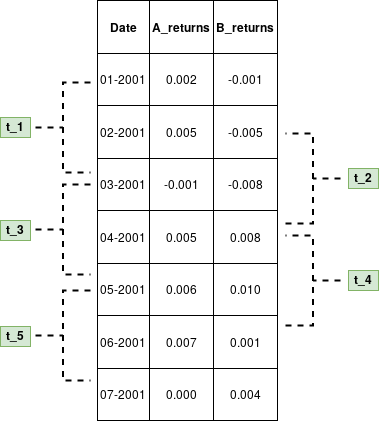
\includegraphics[width=.50\textwidth]{Bilder/rolling_window.png}
    \caption{Illustration of the rolling-window approach for a time-series containing seven time-steps filled with mock-data. Five subsets of length 3 divide the time-series.}
    \label{fig:rolling_window}
  \end{center}
\end{figure}
This approach is schematically described in figure \ref{fig:rolling_window}.\\

Finally, for each subset $t_i$, the weights are computed by solving the system of linear equations as in \ref{eq:9}. Out-of-sample excess returns are then calculated using the actual excess returns of the $i+1$'th time-step in an attempt to validate if a prediction in the past had been successful.\\

Lastly, the out-of-sample returns' arithmetic mean $\hat{\mu}$is devided by its standard deviation $\hat{\sigma}$ to derive the out-of-sample Sharpe ratio like so:
\begin{equation}\label{eq:out-of-sample-sharpe}
\hat{SR} = \frac{\hat{\mu}}{\hat{\sigma}}
\end{equation}

\subsection{Implementation}
In this section we want to display and discuss the implementation of the approach described in the previous chapter in the R programming language. We will compute several performance measures of the Minimal Variance Portfolio we're about to derive from the data.

\subsection{Datasets and data preparation}
The first dataset upon which this analysis is based is called "Ten sector portfolios of the S\&P 500 and the US equity market portfolio". It has been created by Roberto Wessels and was obtained from Mendeley Data\footnote{Data can be downloaded \href{https://data.mendeley.com/datasets/ndxfrshm74/3}{here}. It's also attached to this report.}. Note that for this dataset, it is necessary to substract the Treasury Bill-rates from each entry to obtain adjusted returns stripped of the risk-free rate. We call this dataset \textbf{TSP}.\\

The other dataset concerned is provided by Kenneth French and downloaded from his website\footnote{The dataset from Kenneth Frenchs' website can be downloaded \href{http://mba.tuck.dartmouth.edu/pages/faculty/ken.french/ftp/F-F_Research_Data_Factors_CSV.zip}{here} and is also attached to this report.}. The dataset is called "SMB and HML portfolios and the US equity market portfolio" and contains the factors "Small Minus Big" (SMB) and "High Minus Low" (HMB) from the Fama-French three-factor model \footnote{For an introduction to the Fama-French three-factor model, see \href{https://en.wikipedia.org/wiki/Fama\%E2\%80\%93French_three-factor_model}{Wikipedia}.} as well as the whole S\&P500 portfolio. We call this dataset short \textbf{SHS} This dataset is already cleared from the risk-free rate, thus a Treasure Bill-rate adjustment is not necessary.

In listing \ref{code:0}, it is showcased how data is imported and loaded into a dataframe. In line 1, the .csv-file containing the data is loaded via the \lstinline|read.csv| function, where a separator as well as the header-parameter are specified. 

\begin{lstlisting}[caption={Loading the data and subtracting the risk-free rate from the columns of returns yields a dataframe containing the matrix of excess-returns.}, label=code:0, frame=single]
return_matrix = read.csv('../ten-roberto-wessels.csv', header=TRUE, sep=',')
sub_return_matrix = subset(return_matrix, select = -c(13))
sub_return_matrix = apply(sub_return_matrix[,-1], 2, '-', return_matrix[,13])
return_matrix = cbind(return_matrix$Date, sub_return_matrix)
colnames(return_matrix)[1] = 'Date'
\end{lstlisting}
In case of dataset TSP, it is necessary to subtract the risk-free rate from the returns. To do this, a subset of the return\_matrix is created in line 2, excluding the monthly risk-free rate which is stored in column 13 of the return\_matrix. In line 3, the risk-free rate is sutracted from every column the return\_matrix' subset, except for the column containing the date. Line 4 shows the reconstruction of the return\_matrix, now containing risk-free returns. After the dates' column-name has been reset in line 5, the return\_matrix now contains only risk-free returns. 

\subsubsection{Computing the in-sample Sharpe ratio}
A very basic way of measuring portfolio performance is provided by the in-sample Sharpe ratio. By setting $\tau = \lbrace 1, 2, \dots, T \rbrace$, the entire time-series is considered when computing the covariance matrix of the matrix of excess-returns $\Sigma_t$, effectively removing the weight-vectors' time-dependency. \\

Following the procedure leading to the system of linear equations in equation\ref{eq:9}, we first compute a covariance matrix of the entire risk-free return-matrix. Line 1 of listing \ref{code:is-sharpe-ratio} does just this, excluding the column containing the time-series dates. A vector of dimension equal to the amount of assets listed in the return\_matrix is constructed, where every component of the vector equals one.\\

\begin{lstlisting}[caption={This example shows how the in-sample Sharpe ratio for a matrix of expected returns, computed in the R programming language.}, label=code:is-sharpe-ratio, frame=single]
cov_return_matrix = cov(return_matrix[,-1])
b = vector(length=nA) + 1
weights = solve(cov_benchmark_matrix, b)
weights = weights/abs(sum(weights))
mean_returns = data.matrix(apply(benchmark_matrix[,-1], 2, mean))
weights = data.matrix(weights)
Sharpe_ratio_IS = t(mean_returns) %*% weights / sqrt(t(weights)%*%cov_benchmark_matrix%*%weights)
print(Sharpe_ratio_IS)
\end{lstlisting}

Line 3 of listing \ref{code:is-sharpe-ratio} uses the \lstinline|solve()| function to solve the linear equation by inverting the covariance matrix. The resulting \lstinline|weights|-vector is normalized in line 4. A vector containing the mean-values of \lstinline|return_matrix| is created in line 5 and the \lstinline|weights|-vector is converted to a data.matrix in line 6. This is done to facilitate the vector- and matrix-multiplication performed in line 7 to calculate the in-sample Sharpe ratio according to equation \ref{eq:in-sample-sharpe}, which is printed in line 7.\\

\subsection{Computing the out-sample Sharpe ratio} \label{subsec:minVar-out-sample-sharpe}
For computing the out-sample Sharpe ratio as described in section \ref{subsec:out-sample-sharpe-ratio}, the approach for deriving the in-sample Sharpe ratio needs to be altered to incorporate time-dependency. \\

Considering listing \ref{code:os-sharpe-ratio}, in lines 1 and 2, the number of assets as well as the length of the time-series are assigned respectively. \lstinline|M| contains the length of the rolling-sample, the iterator-variable \lstinline|t| is initialized in line 4 and adjusted to \lstinline|M|.\\

\begin{lstlisting}[caption={Computing the out-sample Sharpe ratio from the matrix of expected returns in R.}, label=code:os-sharpe-ratio, frame=single]
nA = dim(return_matrix[,-1])[2] # number of assets
T = dim(return_matrix)[1] # no of months
M = 120 # size of rolling-sample
t = M + 1 # adjust t_0 to size of rolling-sample
while (t <= T - 1) {
  tStart = t - M 
  tEnd = t 
  return_matrix_future = return_matrix[c(tEnd+1),] 
  cov_return_matrix_t = cov(data.matrix(return_matrix[c(tStart:tEnd),-1])) 
  b_t = vector(length=nA) + 1 
  x_t = solve(cov_return_matrix_t, b_t) 
  x_t = x_t/sum(x_t)
  
  if(t == M+1) { 
    history_of_weights = data.frame(t(x_t))
    mu = data.frame(return_matrix[,1][t], x_t %*% return_matrix_future[-1])
  }
  else {
    history_of_weights = rbind(history_of_weights, x_t)
    mu = rbind(mu, data.frame(return_matrix[,1][t], x_t %*% return_matrix_future[-1]))
  }
  t = t+1
}
\end{lstlisting}

In line 5, the sample gets rolling: By setting a \lstinline|while|-loop, we iterate over the whole time-series. The last date included in the rolling-sample is T-1, since it is the last value for which the expected returns of the next month are known. From line 6 to 12, the weights for time t $x_t$ are computed. They are stored in dataframe mu in line 15 and 19 respectively. Meanwhile, the weights are saved in a dataframe in line 15 and 19.

\subsection{Discussion}
To validate the implementations of the minimum-variance portfolio, in this section metrices derived from the data will be compared with results from DeMiguel et al.\cite{DEM09}. Additionally, results will be graphically displayed and compared.\\

\subsubsection{Graphical Analysis}
As a first graphical display of results, a portfolio appreciation graph is constructed by cumulatively summing the returns and scaling them by a factor 100. Is is similar to having invested 100\$ in a specific portfolio at the beginning of the time-series considered. In figure \ref{fig:appreciation_graph}, the portfolio appreciation graph of the minimum variance portfolio, which has been created in previous chapter \ref{subsec:minVar-out-sample-sharpe}, as well as the portfolio appreciation graph of the naive investing strategy are displayed. When applicating a naive investing strategy as in \cite{DEM09}, the weight-vector $w_{naive}$ is of dimension $N$ and every component of $w_{naive}$ is of value $1/N$, where $N$ is the number of assets considered.
\begin{figure}[h]
  \begin{center}
    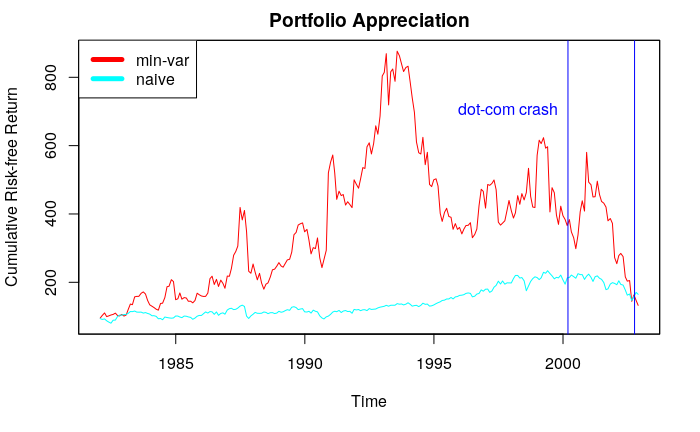
\includegraphics[width=\textwidth]{Bilder/portfolio-appreciation.png}
    \caption{Illustration of the rolling-window approach for a time-series containing seven time-steps filled with mock-data. Five subsets of length 3 divide the time-series.}
    \label{fig:appreciation_graph}
  \end{center}
\end{figure}


\section{Bayes-Stein-Portfolio}
Lorem ipsum dolor sit amet, consetetur sadipscing elitr, sed diam nonumy eirmod tempor invidunt ut labore et dolore magna aliquyam erat, sed diam voluptua. At vero eos et accusam et justo duo dolores et ea rebum. Stet clita kasd gubergren, no sea takimata sanctus est Lorem ipsum dolor sit amet. Lorem ipsum dolor sit amet, consetetur sadipscing elitr, sed diam nonumy eirmod tempor invidunt ut labore et dolore magna aliquyam erat, sed diam voluptua. At vero eos et accusam et justo duo dolores et ea rebum. Stet clita kasd gubergren, no sea takimata sanctus est Lorem ipsum dolor sit amet.
\subsection{Theory}
Lorem ipsum dolor sit amet, consetetur sadipscing elitr, sed diam nonumy eirmod tempor invidunt ut labore et dolore magna aliquyam erat, sed diam voluptua. At vero eos et accusam et justo duo dolores et ea rebum. Stet clita kasd gubergren, no sea takimata sanctus est Lorem ipsum dolor sit amet. Lorem ipsum dolor sit amet, consetetur sadipscing elitr, sed diam nonumy eirmod tempor invidunt ut labore et dolore magna aliquyam erat, sed diam voluptua. At vero eos et accusam et justo duo dolores et ea rebum. Stet clita kasd gubergren, no sea takimata sanctus est Lorem ipsum dolor sit amet.
\subsection{Execution}
Lorem ipsum dolor sit amet, consetetur sadipscing elitr, sed diam nonumy eirmod tempor invidunt ut labore et dolore magna aliquyam erat, sed diam voluptua. At vero eos et accusam et justo duo dolores et ea rebum. Stet clita kasd gubergren, no sea takimata sanctus est Lorem ipsum dolor sit amet. Lorem ipsum dolor sit amet, consetetur sadipscing elitr, sed diam nonumy eirmod tempor invidunt ut labore et dolore magna aliquyam erat, sed diam voluptua. At vero eos et accusam et justo duo dolores et ea rebum. Stet clita kasd gubergren, no sea takimata sanctus est Lorem ipsum dolor sit amet.
\subsection{Discussion}
Lorem ipsum dolor sit amet, consetetur sadipscing elitr, sed diam nonumy eirmod tempor invidunt ut labore et dolore magna aliquyam erat, sed diam voluptua. At vero eos et accusam et justo duo dolores et ea rebum. Stet clita kasd gubergren, no sea takimata sanctus est Lorem ipsum dolor sit amet. Lorem ipsum dolor sit amet, consetetur sadipscing elitr, sed diam nonumy eirmod tempor invidunt ut labore et dolore magna aliquyam erat, sed diam voluptua. At vero eos et accusam et justo duo dolores et ea rebum. Stet clita kasd gubergren, no sea takimata sanctus est Lorem ipsum dolor sit amet.

\section{Sample-based mean-variance-Portfolio}
Lorem ipsum dolor sit amet, consetetur sadipscing elitr, sed diam nonumy eirmod tempor invidunt ut labore et dolore magna aliquyam erat, sed diam voluptua. At vero eos et accusam et justo duo dolores et ea rebum. Stet clita kasd gubergren, no sea takimata sanctus est Lorem ipsum dolor sit amet. Lorem ipsum dolor sit amet, consetetur sadipscing elitr, sed diam nonumy eirmod tempor invidunt ut labore et dolore magna aliquyam erat, sed diam voluptua. At vero eos et accusam et justo duo dolores et ea rebum. Stet clita kasd gubergren, no sea takimata sanctus est Lorem ipsum dolor sit amet.
\subsection{Theory}
Lorem ipsum dolor sit amet, consetetur sadipscing elitr, sed diam nonumy eirmod tempor invidunt ut labore et dolore magna aliquyam erat, sed diam voluptua. At vero eos et accusam et justo duo dolores et ea rebum. Stet clita kasd gubergren, no sea takimata sanctus est Lorem ipsum dolor sit amet. Lorem ipsum dolor sit amet, consetetur sadipscing elitr, sed diam nonumy eirmod tempor invidunt ut labore et dolore magna aliquyam erat, sed diam voluptua. At vero eos et accusam et justo duo dolores et ea rebum. Stet clita kasd gubergren, no sea takimata sanctus est Lorem ipsum dolor sit amet.
\subsection{Execution}
Lorem ipsum dolor sit amet, consetetur sadipscing elitr, sed diam nonumy eirmod tempor invidunt ut labore et dolore magna aliquyam erat, sed diam voluptua. At vero eos et accusam et justo duo dolores et ea rebum. Stet clita kasd gubergren, no sea takimata sanctus est Lorem ipsum dolor sit amet. Lorem ipsum dolor sit amet, consetetur sadipscing elitr, sed diam nonumy eirmod tempor invidunt ut labore et dolore magna aliquyam erat, sed diam voluptua. At vero eos et accusam et justo duo dolores et ea rebum. Stet clita kasd gubergren, no sea takimata sanctus est Lorem ipsum dolor sit amet.
\subsection{Discussion}
Lorem ipsum dolor sit amet, consetetur sadipscing elitr, sed diam nonumy eirmod tempor invidunt ut labore et dolore magna aliquyam erat, sed diam voluptua. At vero eos et accusam et justo duo dolores et ea rebum. Stet clita kasd gubergren, no sea takimata sanctus est Lorem ipsum dolor sit amet. Lorem ipsum dolor sit amet, consetetur sadipscing elitr, sed diam nonumy eirmod tempor invidunt ut labore et dolore magna aliquyam erat, sed diam voluptua. At vero eos et accusam et justo duo dolores et ea rebum. Stet clita kasd gubergren, no sea takimata sanctus est Lorem ipsum dolor sit amet.
